\documentclass{article}
\pdfpagewidth=8.5in
\pdfpageheight=11in
\usepackage{ijcai26} % official IJCAI--ECAI 2026 style
\usepackage{times}
\usepackage{soul}
\usepackage[utf8]{inputenc}
\usepackage{url}
\usepackage[hidelinks]{hyperref}
\urlstyle{same}
\usepackage{graphicx}
% Support compiling from this directory, from parent, or when invoked with a relative path
\graphicspath{{Figure/}{./Figure/}{../Figure/}{FormattingGuidelines-IJCAI-ECAI-26/Figure/}}
\usepackage[font=small]{caption}
\usepackage{subcaption}
\usepackage{amsmath,amssymb}
\usepackage{booktabs}
\usepackage{multirow}
\usepackage[switch]{lineno}
\hfuzz=5pt
\hbadness=10000
\emergencystretch=1em

\pdfinfo{
/TemplateVersion (IJCAI.2026.0)
}

\linenumbers

\title{Set-Aware Bias-Robust Filtering for Biased Recursive Estimation}

\author{
Anonymous Submission
\affiliations
Affiliations withheld for double-blind review
\emails
anonymous@ijcai
}

\begin{document}

\maketitle

\begin{abstract}
Biased recursive estimation suffers from bias floors, collapse under strong regularization, and non-monotonic pairwise bias that defeats pointwise filters. We study a set-aware bias-robust filter with dual heads that jointly reweight samples and predict a corrective shift. Under bounded systematic bias and strong contraction, we prove the expected error is uniformly ultimately bounded. Experiments on synthetic bias sources, high-dimensional regimes, recursive regression, and MNIST drift show the method breaks bias floors (up to $10\times$), improves data efficiency, and handles ripple-shaped bias that pointwise/mean filters miss.
\end{abstract}

\section{Introduction}
Recursive estimators drift when training data, priors, or regularizers introduce systematic bias. Reweighting alone cannot remove bias floors, and correction-only methods can explode under skewed sets. We propose a set-aware filter that learns pairwise structure within candidate sets and adds a corrective head to pull estimates toward bias-free solutions.

\textbf{Contributions}
\begin{itemize}
    \item A biased-error model with a deterministic bias term and a proof of uniform ultimate boundedness (UUB) under strong contraction plus bounded bias/noise.
    \item A set-aware dual-head filter that jointly reweights and corrects, with losses encouraging contraction, effective sample size (ESS), and stable corrections.
    \item An empirical study across eight settings (Exp1--Exp8) showing bias breaking, data efficiency, and robustness to non-monotonic/ripple bias and visual drift.
\end{itemize}

\section{Related Work}
We build on work in importance reweighting for biased estimation, bias-correction filters, and set/attention-based architectures that model pairwise relations. Unlike pointwise MLP filters that average features, our design leverages set-level attention to detect non-monotonic pairwise bias while keeping a correction head to collapse bias floors in recursive updates.

\section{Theory}
We model biased error dynamics as
\begin{equation}
    \mathbf{e}_{t+1} = A(\mathbf{e}_t)\mathbf{e}_t + \mathbf{b}(\mathbf{e}_t) + \xi_t,
\end{equation}
where $\mathbf{e}_t = \theta_t - \theta^\ast$, $A(\cdot)$ is a state-dependent contraction, $\mathbf{b}(\cdot)$ is deterministic bias, and $\xi_t$ is zero-mean noise.

\textbf{Assumption (Strong contraction).} $\exists P \succ 0, c(\mathbf{e})\in[0,1)$ s.t. $A(\mathbf{e})^\top P A(\mathbf{e}) \preceq (1-c(\mathbf{e}))P$ and $c(\mathbf{e})V(\mathbf{e}) \ge f(V(\mathbf{e}))$ for $V(\mathbf{e})=\mathbf{e}^\top P\mathbf{e}$ and convex $f$.

\textbf{Assumption (Bounded bias/noise).} $\sup_{\mathbf{e}}\|\mathbf{b}(\mathbf{e})\|_P \le \beta$ and $\mathbb{E}[\xi_t^\top P \xi_t] \le \sigma^2$, with total disturbance energy $\epsilon = \beta^2 + \sigma^2$.

\textbf{Step 1: conditional energy.} Expanding $\mathbb{E}[V(\mathbf{e}_{t+1}) \mid \mathbf{e}_t]$ gives
\begin{align}
    \mathbb{E}[V_{t+1}\mid\mathbf{e}_t] &= (A\mathbf{e}_t)^\top P (A\mathbf{e}_t) + \mathbf{b}^\top P\mathbf{b} + \mathbb{E}[\xi_t^\top P\xi_t] \nonumber\\
    &\quad + 2(A\mathbf{e}_t)^\top P\mathbf{b} \nonumber\\
    &\le (A\mathbf{e}_t)^\top P (A\mathbf{e}_t) + \epsilon + 2(A\mathbf{e}_t)^\top P\mathbf{b}.
\end{align}

\textbf{Step 2: cross-term bounding.} Applying Young's inequality $2x^\top Py \le \eta x^\top Px + \tfrac{1}{\eta}y^\top Py$ with $x=A\mathbf{e}_t,y=\mathbf{b}$,
\begin{equation}
    \mathbb{E}[V_{t+1}\mid\mathbf{e}_t] \le (1+\eta)(A\mathbf{e}_t)^\top P(A\mathbf{e}_t) + \left(1+\tfrac{1}{\eta}\right)\beta^2 + \sigma^2.
\end{equation}
Using strong contraction, $(A\mathbf{e}_t)^\top P(A\mathbf{e}_t) \le V_t - f(V_t)$.

\textbf{Step 3: unconditional recursion.} Let $x_t = \mathbb{E}[V(\mathbf{e}_t)]$. Jensen gives $\mathbb{E}[f(V_t)] \ge f(x_t)$, so
\begin{equation}
    x_{t+1} \le (1+\eta)\bigl(x_t - f(x_t)\bigr) + C_\eta,\quad C_\eta = \left(1+\tfrac{1}{\eta}\right)\beta^2 + \sigma^2.
\end{equation}
Error decreases when $f(x_t) > \tfrac{\eta}{1+\eta}x_t + \tfrac{C_\eta}{1+\eta}$.

\textbf{Theorem (UUB under bias).} The expected error is uniformly ultimately bounded: $x_t$ converges to $\mathcal{S}=\{x \ge 0 \mid x \le R^\ast\}$ where $R^\ast$ solves $f(x)=\tfrac{\eta}{1+\eta}x + \tfrac{C_\eta}{1+\eta}$. Bias and noise define a finite radius; the filter contracts trajectories back inside $\mathcal{S}$ rather than drifting or collapsing. When $f(\cdot)$ grows faster than the linear right-hand side, the contraction term dominates for $x_t>R^\ast$, pulling the system back, while inside $R^\ast$ the disturbance limits further decay.

\section{Method}
\textbf{Set encoder.} A transformer over the candidate set encodes pairwise and higher-order relations, critical for non-monotonic pairwise bias (e.g., ripple patterns).

\textbf{Dual heads.} (1) Weight head outputs importance weights $w_i$ (softmax, ESS regularization). (2) Correction head predicts $\Delta\phi$ that shifts the aggregated estimate to counter bias. The update is $\hat{\theta}_{t+1} = \sum_i w_i x_i + \Delta\phi$.

\textbf{Loss.} Weighted likelihood/classification + contraction regularizer (encouraging $A(\cdot)$ to be contractive), ESS penalty to avoid degeneracy, and correction regularization to keep $\Delta\phi$ stable. Auxiliary supervision aligns $\Delta\phi$ with observed bias direction when available.

\section{Experiments}
We report eight settings with 6--8 figures; key plots are included below (paths preserved in \texttt{Figure/}).

\textbf{Exp1 Bias sources.} Strong bias (hard $b{=}0.5$, Ridge $\alpha{=}20$, wrong prior) shows bias floors: No Filter tails $\approx$0.997/0.383/0.795, Standard weighting $\approx$0.305/0.025/0.035, ours $\approx$0.076/0.031/0.031 (gen 300). Correction head breaks hard-bias floors; weighting suffices when variance dominates.

\textbf{Exp2 Bias sensitivity.} From \texttt{Table/table\_exp2\_bias\_summary.csv}, the set-aware filter caps tails at $\approx$0.04 even when the systematic bias doubles to 2.0, while Standard rises to 1.85 and No Filter to 2.00. Under prior shift with $n{=}5$ and $\delta{=}20$ (\texttt{Table/table\_exp2\_prior\_summary\_n5.csv}), tails are 7.63 (No), 2.84 (Standard), 0.045 (ours); at $n{=}50$ and $\delta{=}20$ they are 0.44 / 0.44 / 0.045 (\texttt{Table/table\_exp2\_prior\_summary\_n50.csv}). Ridge stress at $\alpha{=}50$ keeps ours at 0.035 vs 1.15 (No) and 1.04 (Standard) (\texttt{Table/table\_exp2\_ridge\_summary.csv}).

\textbf{Exp3 Data efficiency.} Correction recovers large-sample baselines with $10\times$ fewer samples: hard bias $|b|{=}0.5$ tail $\approx$0.031; Ridge $n{=}100$ vs 10k: 0.036 vs 0.0017; Bayes $n{=}5$: ours 0.080 vs unfiltered 0.165.

\textbf{Exp4 Mechanism.} $\Delta\phi$ aligns with bias direction (cos $\approx$0.99), ESS stays $\approx$131--160/160; weights emphasize samples far from biased priors.

\textbf{Exp5 High dimension.} At $d{=}50/100$, set-aware edges out MLP+Corr (tails 0.097/0.146 vs 0.101/0.149); at $d{=}500$, MLP+Corr collapses (17.50) while set-aware stays at 0.74. Weight-only MLP sits around 0.50--0.54.

\textbf{Exp6 Architecture ablation.} Correction-only and set-aware dominate in Bayes (0.051/0.052) and complex bias (0.137/0.138); MLP+Corr collapses on complex (0.537) but is best on Ridge $\alpha{=}10$ (0.054 vs ours 0.058). Weight-only fails across all.

\textbf{Exp7 Ripple bias (pairwise).} Only set-aware attends to non-monotonic pairwise bias; MSE $\approx$0.58 with waveform tracking, while pointwise/MLP give flat predictions (MSE 41/54). Attention maps focus on anomalous pairs; t-SNE shows structured latent.

\textbf{Exp7 Recursive regression (real).} On California housing recursive Ridge, test MSE drops from $\approx$5.68 (No) to 4.86 (ours, $14\%$ relative), with larger parameter norms preserved.

\textbf{Exp8 MNIST drift.} Under 5$^\circ$ per-generation rotation, ours slashes test MSE to $\approx 1.2{\times}10^{-4}$ vs 0.0325 (No) and 0.0308 (MLP). Corrections grow norm to track drift while reweighting alone underfits.

Key tail metrics (numbers below; source CSVs in \texttt{Table/}).

\begin{table}[t]
    \centering
    \footnotesize
    \begin{tabular}{lccc}
    \toprule
    Exp1 tail (gen 300) & No & Standard & Ours \\
    \midrule
    Hard bias $|b|{=}0.5$ & 0.997 & 0.305 & 0.076 \\
    Ridge $\alpha{=}20$ & 0.383 & 0.025 & 0.031 \\
    Bayes $\sigma{=}0.2,n{=}20$ & 0.795 & 0.035 & 0.031 \\
    \bottomrule
    \end{tabular}
    \caption{Exp1 bias sources (lower is better); see Table/table\_exp1\_tail.csv.}
    \label{tab:exp1}
\end{table}

\begin{table}[t]
    \centering
    \footnotesize
    \begin{tabular}{lccc}
    \toprule
    Exp3 tail (gen 200) & Big-sample & Small+NoFilt & Small+Ours \\
    \midrule
    Hard bias $|b|{=}0.5$ & 0.500 & 0.504 & 0.031 \\
    Ridge $n{=}100$ & 0.0017 & 0.115 & 0.0355 \\
    Bayes $n{=}5$ & 0.0012 & 0.165 & 0.0798 \\
    \bottomrule
    \end{tabular}
    \caption{Exp3 data efficiency tails; see Table/table\_exp3\_data\_eff\_tail.csv.}
    \label{tab:exp3}
\end{table}

\begin{table}[t]
    \centering
    \footnotesize
    \begin{tabular}{lcccc}
    \toprule
    Exp5 tail (n=50) & No & MLP (w) & MLP+Corr & Set-aware \\
    \midrule
    $d{=}50$ & 0.540 & 0.502 & 0.101 & 0.097 \\
    $d{=}100$ & 0.571 & 0.503 & 0.149 & 0.146 \\
    $d{=}500$ & 0.805 & 0.541 & 17.50 & 0.741 \\
    \bottomrule
    \end{tabular}
    \caption{Exp5 high-dimensional tails; see Table/table\_exp5\_tail\_summary.csv.}
    \label{tab:exp5}
\end{table}

\begin{table}[t]
    \centering
    \footnotesize
    \begin{tabular}{lcccc}
    \toprule
    Exp6 tail & Weight-only & Corr-only & MLP+Corr & Set-aware \\
    \midrule
    Bayes $n{=}5$ & 1.456 & 0.051 & 0.263 & 0.052 \\
    Ridge $\alpha{=}10$ & 1.254 & 0.059 & 0.054 & 0.058 \\
    Complex bias & 0.239 & 0.137 & 0.537 & 0.138 \\
    \bottomrule
    \end{tabular}
    \caption{Exp6 ablations; see Table/table\_exp6\_*.csv.}
    \label{tab:exp6}
\end{table}

\begin{table}[t]
    \centering
    \footnotesize
    \begin{tabular}{lcccc}
    \toprule
    Task (tail gen) & Method & Test MSE & Param norm & Time (s) \\
    \midrule
    Recursive regression (300) & No & 5.683 & 0.040 & 19.16 \\
     & Ours & 4.859 & 1.551 & 19.16 \\
    MNIST drift (200) & No & 0.0325 & 2.853 & 100.34 \\
     & MLP (w) & 0.0308 & 2.923 & 100.34 \\
     & Ours & $1.2\\times 10^{-4}$ & 7.007 & 100.34 \\
    \bottomrule
    \end{tabular}
    \caption{Exp7/8 tails; see Table/table\_exp7\_recursive\_tail.csv and Table/table\_exp8\_mnist\_tail.csv.}
    \label{tab:exp78}
\end{table}

\begin{figure}[t]
    \centering
    \begin{subfigure}{0.48\linewidth}
        \centering
        \includegraphics[width=\linewidth]{exp1_1.1_const.png}
        \caption{Exp1 bias sources}
    \end{subfigure}
    \hfill
    \begin{subfigure}{0.48\linewidth}
        \centering
        \includegraphics[width=\linewidth]{exp2_2.1_trajs_by_method.png}
        \caption{Exp2 sensitivity}
    \end{subfigure}
    \caption{Bias floors and sensitivity across sources/strengths.}
    \label{fig:exp12}
\end{figure}

\begin{figure}[t]
    \centering
    \begin{subfigure}{0.48\linewidth}
        \centering
        \includegraphics[width=\linewidth]{exp3_fig_A_breaking_floor.png}
        \caption{Breaking bias floor}
    \end{subfigure}
    \hfill
    \begin{subfigure}{0.48\linewidth}
        \centering
        \includegraphics[width=\linewidth]{exp3_fig_B_data_efficiency.png}
        \caption{Data efficiency}
    \end{subfigure}
    \caption{Exp3: correction enables bias breaking with $10\times$ fewer samples.}
    \label{fig:exp3}
\end{figure}

\begin{figure}[t]
    \centering
    \begin{subfigure}{0.48\linewidth}
        \centering
        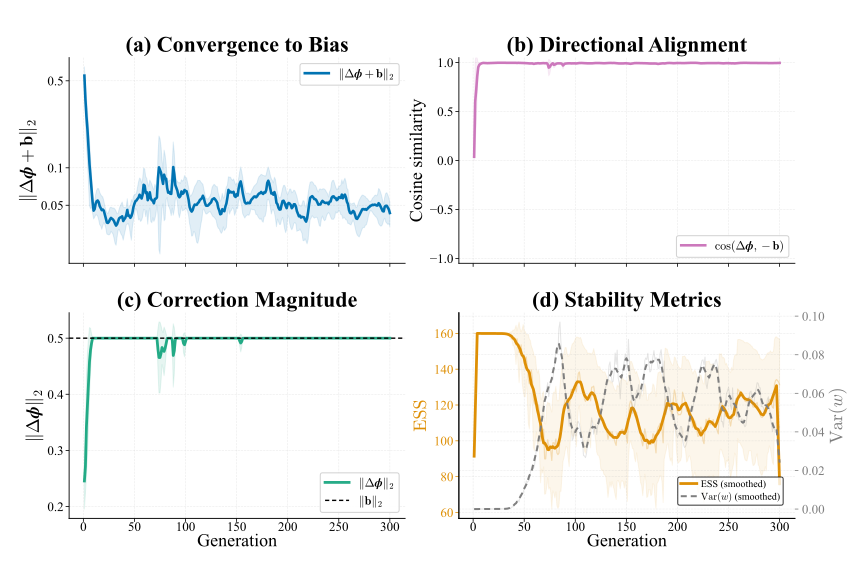
\includegraphics[width=\linewidth]{exp4_4.1_base.png}
        \caption{Mechanism (Exp4)}
    \end{subfigure}
    \hfill
    \begin{subfigure}{0.48\linewidth}
        \centering
        \includegraphics[width=\linewidth]{exp5_tail_vs_dim.png}
        \caption{High-$d$ scaling (Exp5)}
    \end{subfigure}
    \caption{Mechanism visualization and high-dimensional behavior.}
    \label{fig:exp45}
\end{figure}

\begin{figure}[t]
    \centering
    \begin{subfigure}{0.48\linewidth}
        \centering
        \includegraphics[width=\linewidth]{exp6_trajs.png}
        \caption{Ablation (Exp6)}
    \end{subfigure}
    \hfill
    \begin{subfigure}{0.48\linewidth}
        \centering
        \includegraphics[width=\linewidth]{exp7_combined.png}
        \caption{Ripple bias (Exp7)}
    \end{subfigure}
    \caption{Dissecting architecture choices and pairwise bias handling.}
    \label{fig:exp67}
\end{figure}

\begin{figure}[t]
    \centering
    \begin{subfigure}{0.48\linewidth}
        \centering
        \includegraphics[width=\linewidth]{exp7_curves.png}
        \caption{Recursive regression}
    \end{subfigure}
    \hfill
    \begin{subfigure}{0.48\linewidth}
        \centering
        \includegraphics[width=\linewidth]{exp8_curves.png}
        \caption{MNIST drift}
    \end{subfigure}
\caption{Real-data recursion and visual drift (Exp7/8).}
\label{fig:exp78}
\end{figure}

\section{Discussion}
Set-aware correction is most valuable when bias is strong, non-monotonic, or when data are scarce. In high dimensions with low sample counts, pointwise MLP+Corr is competitive, suggesting the set encoder should be scaled or sparsified. Balancing weight and correction losses is essential to avoid ESS collapse or over-correction.

\section{Conclusion}
We presented a set-aware dual-head filter for biased recursive estimation, proved UUB under bounded bias, and demonstrated substantial bias breaking, data efficiency gains, and robustness to ripple and visual drift. Future work includes scalable encoders for very high dimensions and automatic loss balancing for weight/correction synergy.

\appendix
\section{Extended Theory (Derivation)}
We restate the full derivation (adapted from ``Uniform Ultimate Boundedness under Biased Estimation''):
\begin{itemize}
    \item \textbf{Model.} $\mathbf{e}_{t+1} = A(\mathbf{e}_t)\mathbf{e}_t + \mathbf{b}(\mathbf{e}_t) + \xi_t$, with $A(\cdot)$ state-dependent contraction, deterministic bias $\mathbf{b}(\cdot)$, zero-mean noise $\xi_t$.
    \item \textbf{Assumptions.} (i) Strong contraction: $\exists P\succ 0, c(\mathbf{e})\in[0,1)$ s.t. $A(\mathbf{e})^\top P A(\mathbf{e}) \preceq (1-c(\mathbf{e}))P$ and $c(\mathbf{e})V(\mathbf{e})\ge f(V(\mathbf{e}))$, $V(\mathbf{e})=\mathbf{e}^\top P\mathbf{e}$. (ii) Bounded bias/noise: $\sup_{\mathbf{e}}\|\mathbf{b}(\mathbf{e})\|_P \le \beta$, $\mathbb{E}[\xi_t^\top P\xi_t]\le\sigma^2$.
    \item \textbf{Step 1 (conditional energy).} $\mathbb{E}[V_{t+1}\mid\mathbf{e}_t] = (A\mathbf{e}_t)^\top P (A\mathbf{e}_t) + \mathbf{b}^\top P\mathbf{b} + \mathbb{E}[\xi_t^\top P\xi_t] + 2(A\mathbf{e}_t)^\top P\mathbf{b}$.
    \item \textbf{Step 2 (cross term).} Young with parameter $\eta>0$: $2(A\mathbf{e}_t)^\top P\mathbf{b} \le \eta (A\mathbf{e}_t)^\top P(A\mathbf{e}_t) + \tfrac{1}{\eta}\beta^2$, giving $\mathbb{E}[V_{t+1}\mid\mathbf{e}_t] \le (1+\eta)(A\mathbf{e}_t)^\top P(A\mathbf{e}_t) + C_\eta$, $C_\eta=\left(1+\tfrac{1}{\eta}\right)\beta^2+\sigma^2$.
    \item \textbf{Step 3 (apply contraction).} $(A\mathbf{e}_t)^\top P(A\mathbf{e}_t) \le V_t - f(V_t)$, so $\mathbb{E}[V_{t+1}\mid\mathbf{e}_t] \le (1+\eta)(V_t - f(V_t)) + C_\eta$.
    \item \textbf{Step 4 (unconditional recursion).} Let $x_t=\mathbb{E}[V_t]$. Jensen yields $x_{t+1} \le (1+\eta)(x_t - f(x_t)) + C_\eta$ and the decrease condition $f(x_t) > \tfrac{\eta}{1+\eta}x_t + \tfrac{C_\eta}{1+\eta}$.
    \item \textbf{UUB radius.} $x_t$ converges to $\mathcal{S}=\{x\ge 0\mid x\le R^\ast\}$ where $R^\ast$ is the largest root of $f(x)=\tfrac{\eta}{1+\eta}x + \tfrac{C_\eta}{1+\eta}$. For $x_t>R^\ast$, contraction dominates and pulls back; inside $R^\ast$, disturbance energy limits further decay.
\end{itemize}

\section{Additional Results}
The appendix can include full figures/tables for Exp1--Exp8, ablations, and hyperparameter details, as space allows.

\bibliographystyle{named}
\bibliography{ijcai26}

\end{document}
